\documentclass{article}
\usepackage{titlesec}
\usepackage{lipsum}
\usepackage{hyperref}
\usepackage{graphicx}
\usepackage{appendix}
\usepackage[left=1 in,right=1 in,top=1 in,bottom=1 in]{geometry}

% Remove the red boxes around links
\hypersetup{
    colorlinks=true,
    linkcolor=black,
    citecolor=black,
    urlcolor=blue
}


\titleformat{\section}[hang]{\normalfont\scshape\Large\bfseries}{\thesection}{1em}{}
\titleformat{\subsection}[hang]{\normalfont\scshape\large\bfseries}{\thesubsection}{1em}{}
\titleformat{\subsubsection}[hang]{\normalfont\scshape\normalsize\bfseries}{\thesubsubsection}{1em}{}

\begin{document}

% Title Page
\begin{titlepage}
    \centering
    
\includegraphics[width=0.8\textwidth]{image.jpeg}\par % Adjust the width as needed
     \vspace{2cm}
    {\scshape\Large SOEN 6481: TAS REPORT \par}
    \vspace{1.5cm}
    {\scshape\Huge Topic 58: How should I manage adoption of new technologies or processes in my projects?\par}
    \vspace{1.5cm}
    {\large Advisor: Professor Pankaj Kamthan\par}
    \vspace{1.5cm}
    {\large By: Konark Shah (Student ID: 40232277)\par}
    \vspace{1cm}
    {\large \today\par}
\end{titlepage}

\tableofcontents

\newpage

\section*{Abstract}
This Topic Analysis and Synthesis paper navigates the complexities of managing the adoption of new technologies or processes in projects, considering project nature and team experience. It emphasizes prudent assessment of costs and benefits, highlighting the significance of analyzing the consequences of maintaining the status quo, transition costs, and anticipated monetary benefits. The importance of conservative planning, aligned with skills and risk considerations, is underscored. Securing buy-in is discussed, emphasizing the presentation of a compelling business case. Challenges in organizations are addressed, suggesting a shift towards social-technical adoption models. The paper concludes by recognizing the challenges and advocating for careful planning, stakeholder engagement, and persuasive communication for successful implementation.

\section{Introduction}
In today's fast-changing tech landscape, it's crucial for companies to keep up with the competition by adopting and integrating new technologies into their existing products. Making the right decisions in this process is complex and can make or break a new product. To navigate this terrain successfully, one must consider a range of factors, including the nature of the ongoing project, the team's experience and skill set, communication strategies with stakeholders, and the pivotal step of securing approval from top management. This thesis seeks to unravel the complexities surrounding this crucial decision-making process, offering insights into the managerial intricacies involved in the successful adoption of new technologies or processes within projects.


\subsection{Motivation}
This thesis is motivated by a keen interest in unraveling the complexities of adopting new technology and procedures. Recognizing that understanding this complexity is not just beneficial but essential for successful project navigation, the thesis aims to shed light on practical approaches for managing the adoption of new technologies. It aspires to offer valuable insights for project managers, helping them strike a delicate balance between innovation and seamless project execution.

\subsection{Problem Statement}
The fundamental issue addressed in this paper is the successful management of new technology or process adoption within project environments. The complexity stems from the opposition encountered during major changes, the uncertainties around cost and benefit projections, and the requirement for a proactive strategy to obtain buy-in from contributors and stakeholders. Prudent decision-making in this setting necessitates a thorough awareness of the issues at hand, as well as the creation of appropriate mitigation methods.

\subsection{Research Questions}
\begin{enumerate}
    \item[Q1:] How can project leaders efficiently assess the costs and benefits of adopting new technologies or processes, including estimating the consequences of maintaining the status quo?
    
    \item[Q2:] What strategies help project leaders plan for team skills, knowledge, and resistance when implementing major changes in a project?
    
    \item[Q3:] What elements make a business case persuasive, and how can project leaders tailor communication to align with the interests of stakeholders?
    
    \item[Q4:] How do project managers manage risks and uncertainties in adopting new technologies or processes, and what role does contingency planning play in successful implementation?
\end{enumerate}


---
\subsection{Critical Thinking}

The research questions mark a pivotal stage in investigating the challenges of implementing new technology or processes in projects. Each question represents careful thought on project dynamics, organizational context, and the complexity associated with technological integration.

\subsubsection*{Q1: Efficient Assessment of Costs and Benefits}

For the first question (Q1), it focuses on the pragmatic aspects of project leadership. It aims to understand how project leaders can efficiently assess costs and benefits, balancing the existing state against potential advancements.

\subsubsection*{Q2: Strategies for Planning in the Face of Change}

The second question (Q2) addresses the necessity for strategic planning in implementing major changes. This inquiry seeks strategies for project leaders to navigate challenges related to team skills, knowledge, and resistance during technological integration.

\subsubsection*{Q3: Persuasive Business Cases and Stakeholder Alignment}

The third question (Q3) stems from recognizing communication’s role in technology adoption. Exploring the elements that make a business case persuasive, emphasizing stakeholder alignment as crucial for successful integration.

\subsubsection*{Q4: Risk Management and Contingency Planning}

The fourth question (Q4) underscores our commitment to addressing uncertainties tied to technological adoption. The aim is to uncover how project managers can proactively manage risks, emphasizing the role of contingency planning in ensuring successful implementation.
\newline

\noindent In formulating these research questions, careful consideration was given to project dynamics, team experience, and the broader impact of technology integration. Each question aims to reveal practical insights into the effective management of projects in the evolving tech landscape. The subsequent section will outline clear objectives, providing a road-map for the research journey.



\subsection{Objectives}

The objectives of this investigation are to:

\begin{itemize}
  \item Evaluate the impact of project nature and team experience on technology and process adoption.
  \item Analyze the costs of staying with the current methods and transitioning to new technologies or processes.
  \item Determine the monetary benefits of adopting new technologies or processes.
  \item Identify effective techniques for overcoming internal organizational resistance to the adoption of new technologies.
  \item Recognize and analyze the limitations of various solutions and explore their future scope.
\end{itemize}

\noindent This research aims to provide valuable insights and practical techniques for project leaders, managers, and stakeholders, enabling them to navigate the complexities of technology adoption in project environments. It addresses inherent difficulties and uncertainties by thoroughly examining key factors associated with the adoption of new technologies or processes.

\section{Background Material}
The adoption and integration of new technology pose a managerial challenge with a substantial impact on overall corporate success. This section delves into the fundamentals, examining the nature of the project change, identifying various factors affected, essential mechanisms for the integration process, and outlining specific conditions that guide their effective utilization. This expertise is particularly valuable for managers overseeing technology integration, offering practical advice on navigating the process within their specific organizational contexts.


\subsection{Nature of the project change and their Impact}
Understanding a project before embracing change involves considering various factors. The primary factor is the organization's level of prior experience with technology integration, commonly referred to as technological maturity. The second factor revolves around assessing the extent to which the new technology contributes to product advancement. This evaluation involves determining whether the technology enhances the existing product's functionality beyond its original scope, thereby generating a strategic advantage. Alternatively, it considers scenarios where the new technology serves as an additional support function without altering the fundamental features of the core mechanical product \cite{reference1}.


\begin{figure}[h]
    \centering
    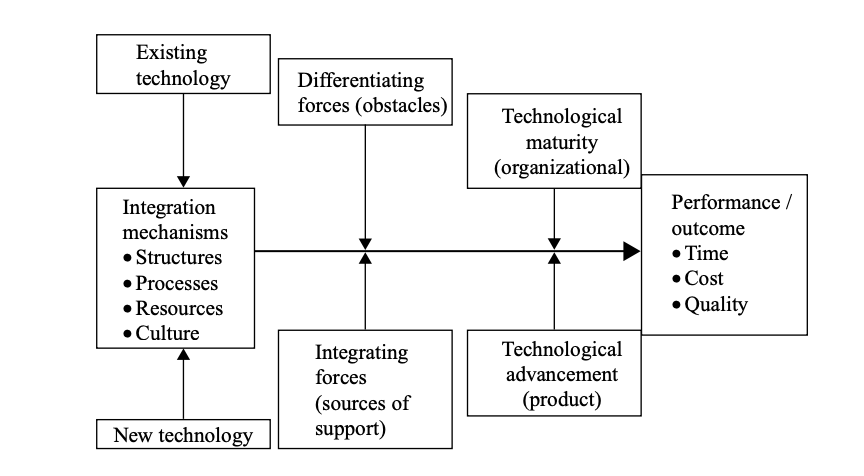
\includegraphics[width=0.8\textwidth]{Figure1.png}
    \caption{Conceptual model of the project change with implications and impact \cite{reference1}.}
    \label{fig:conceptual-model}
\end{figure}

\noindent The model in Figure 1 illustrates various things involved in during the project change and their impacts. Initially understanding the existing technology and the new to-be-adopted technology results in changes to the structures, processes, resources, and culture of the organization. Further into the picture are obstacles (differentiating forces) and sources of support (integrating forces) that influence the process. Finally, understanding the technological maturity of the current product/process and the advancement done to it, streamlining the analysis of their impacts, and taking deliberate steps based on this understanding as a project manager leads to favorable outcomes, benefiting the organization.

\subsection{Role of team experience in technology/process adoption}

The seamless adoption of technology within any project is intricately linked to the collaborative efforts of the involved team. The team's collective motivation, combined with their prior knowledge and skill sets, significantly shapes the trajectory of adoption, creating an environment conducive to successful integration. However, without proper attention, challenges such as resistance to change, gaps in knowledge, a resistant mindset, and a lack of collaboration can impede the technology/process adoption process. As rightly stated, "People's commitment to change increases the chance of successful transformation and decreases the cost of change. It is the most powerful catalyst for changing approach" \cite{reference2}.


\section{Methods \& Methodology}
This section explores methods and methodologies designed to address the challenges associated with technology adoption. The focus is on strategic steps that project managers can employ to ensure the successful adoption of technology. This encompasses effective approaches to mitigate resistance, enhance knowledge transfer, deal with differentiating and integrating forces, foster a positive mindset among the team, and promote collaborative practices, as explained in the above section. Additionally, there will be a delve into the critical aspect of analyzing costs and benefits related to change adoption, securing buy-in, and implementing planning methods. The discussion will be enriched with examples from case studies illustrating how organizations have successfully handled technology adoption using these methods.


\subsection{Analyzing costs and benefits}
In the realm of technology adoption, a thorough evaluation of costs serves as a fundamental pillar in strategic decision-making. These costs, whether direct or indirect, play a pivotal role in shaping a project's trajectory. Aligning benefits with project costs is a decisive factor in determining the viability of technology adoption. Benefits, broadly categorized as tangible and intangible, bring inherent value. Tangible benefits, quantifiable by nature, encompass elements like cost reductions, heightened reliability, and increased productivity. In contrast, intangible benefits, though equally valuable, present a challenge in quantification and often materialize as enhanced business opportunities \cite{reference3}.

\begin{figure}[h]
    \centering
    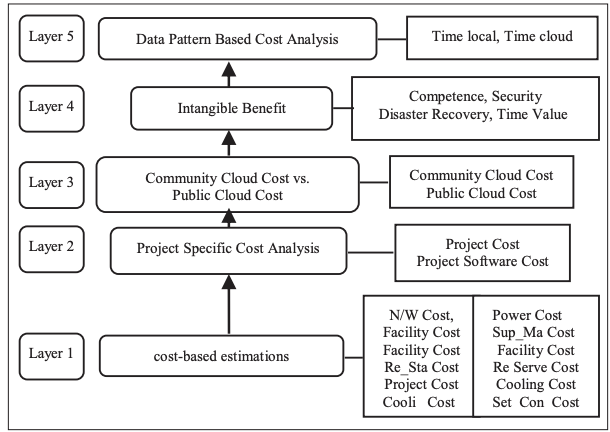
\includegraphics[width=0.7\textwidth]{Figure2.png}
    \caption{Layers of the proposed Cost Benefit Framework \cite{reference3}.}
    \label{fig:conceptual-model}
\end{figure}

\noindent The above explained framework in Figure 2 from \cite{reference3} serves as an example of how organizations approach technology adoption by systematically analyzing costs and benefits:
\begin{itemize}
    \item \textbf{Layer 1:} Direct cost estimation, covering project, facility, setup, real estate(if applicable), power, and related factors.
    \item \textbf{Layer 2:} Project-specific costs within the organization.
    \item \textbf{Layer 3:} Examination of costs linked to choosing a cloud deployment model (public or community).
    \item \textbf{Layer 4:} Focus on intangible benefits like enhanced security, data recovery, and market competitiveness.
    \item \textbf{Layer 5:} Analysis of costs tied to the specific implementation of data retrieval and storage in the cloud.
\end{itemize}

\noindent In conclusion, the illustrated framework serves as a versatile model applicable to various technology adoption processes, offering organizations a comprehensive approach for evaluating costs(direct or indirect) and benefits(tangible and intangible advantages).

\subsection{Estimation Process}
The estimation process aims to establish a systematic approach for assessing resources, efforts, and potential costs linked to adopting new technologies or processes. Employing either bottom-up or top-down approaches based on the software's decomposition structure, the bottom-up method initiates estimates at the lowest level components, aggregating them into higher-level assessments. Conversely, the top-down approach starts with an overview of the entire system, calculating estimates for component parts as relative proportions of the full estimate \cite{reference4}. Both approaches involve a detailed analysis of factors contributing to overall project estimation, such as:
\begin{itemize}
    \item \textbf{Resource Assessment:} Identifying the human resources, skill sets, and expertise required for the successful implementation of the technology.
    \item \textbf{Cost Estimation:} Determining the financial aspects, including direct costs like equipment, software licenses, and indirect costs associated with training and potential downtime.
    \item \textbf{Effort Estimation:} Assessing the amount of effort, in terms of time and labor, required for the adoption process.
    \item \textbf{Timeline and Milestones:} Establishing a timeline for the adoption process, including key milestones and checkpoints for tracking progress.
    \item \textbf{Contingency Planning:} Anticipating potential risks and uncertainties and incorporating contingency plans to mitigate unforeseen challenges.
\end{itemize}

\noindent The estimation process provides project managers with a comprehensive understanding of the resources and costs involved, facilitating better decision-making and planning throughout the technology adoption journey.


\subsection{Verification of Estimates}
Verification of estimates is a pivotal phase in ensuring the reliability of projected costs and benefits within a project. During this critical step, the project manager meticulously examines the provided estimates, aiming to identify any potential changes with a discerning eye. This involves a thorough scrutiny of the underlying data sources, methodologies, and assumptions that form the basis of the estimates.\newline

\noindent The overarching goal is to cultivate a culture of transparency and accuracy, addressing any latent biases or inaccuracies that might be present in the assessments. It is crucial to recognize that the initial and most crucial aspect of verification is related to cost, as it significantly influences the ultimate adoption decision. Empirical validation becomes paramount, as showcased in \cite{reference5}, where four algorithmic models (SLIM, COCOMO, Function Points, and ESTIMACS) proposed as general software-development cost estimators are rigorously validated.\newline

\noindent Beyond cost verification, other facets of the estimation process also demand attention and are covered by some of the algorithm models above including validating the timeline and milestones, ensuring that they align with realistic expectations. Effort verification, a key component, necessitates a comprehensive consideration of the team's skills and previous experiences to provide a realistic evaluation. Additionally, the verification process extends to scrutinizing potential risks and uncertainties, avoiding decisions based on subjective or personal grounds. In essence, the verification of estimates serves as a safeguard, significantly enhancing the credibility of the analysis. This, in turn, facilitates more robust decision-making for project leaders, contributing to the overall success of the technology adoption endeavor.

\subsection{Planning for change and Change Management}
Building on the insights gained from the previous sections and the estimates of the current state of resources, the focus now shifts to the pivotal role of planning for change in technology adoption. This strategic planning involves crucial elements such as resource allocation, the implementation of effective training programs, and the development of robust risk mitigation strategies. \newline


\noindent Change management involves the strategies implemented by management to leverage new methods, models, and technologies in order to gain a competitive advantage for organizations \cite{reference6}. The strategic dimension of change management emphasizes the importance of focusing on people and organizational transformation. \cite{reference7} explains three primary models—Kotter’s change model, Lewin’s change model, and ADKAR’s change management model—are integral to understanding and implementing each phase in change management. Kotter's model revolves around eight key change steps, with a primary emphasis on securing top management buy-in. Lewin's model delineates three significant phases—Unfreeze, Change, Refreeze—prioritizing end-user involvement and the change team. Similarly, ADKAR's model, rooted in the concepts of Awareness, Desire, Knowledge, Ability, and Reinforcement, aligns with Lewin's model's focus \cite{reference7}. \newline

\noindent In conclusion, effective technology adoption hinges on the symbiosis of planning for change and change management. Strategic planning guides resource allocation, training, and risk mitigation, while change management orchestrates organizational transformation. Models like Kotter's, Lewin's, and ADKAR's provide a structured approach. Together, these pillars ensure organizations navigate technological shifts.

\subsection{Securing Buy-In}
This section underlines the need to secure buy-in from management as well as project teams. Presenting a compelling business case underpinned by facts, figures, and concrete benefits is part of a strategic strategy. Aligning the proposed change with results that management and sponsors personally value increases the likelihood of enthusiastic approval. \newline

\noindent Despite the abundance of models and frameworks for IT adoption, challenges persist in organizations. The inadequacy of existing models to address diverse stakeholder perceptions and expectations hinders IT adoption success. Most frameworks are deterministic, neglecting the importance of various stakeholder worldviews in the adoption process. Shifting towards social-technical adoption models is crucial for a comprehensive understanding of IT adoption beyond a linear technological approach. Stakeholders, individuals or groups with organizational interests, engage in a reciprocal interaction influencing both the organization and themselves \cite{reference8}. \newline

\noindent Regular communication, addressing concerns, and showcasing progress are essential methods for sustaining buy-in throughout the adoption process. Furthermore, involving stakeholders in decision-making and seeking their input fosters a sense of ownership, increasing the likelihood of continued support. The commitment to an ongoing dialogue and adaptation to stakeholder feedback significantly contributes to the success of technology adoption initiatives.



\subsection{Overcoming Resistance}
Resistance to change is a natural hurdle in the integration of new technologies or procedures within a project. Effectively addressing and overcoming this resistance is crucial for the successful adoption of innovations. In the preceding sections, various methods have been discussed, covering aspects such as cost-benefit analysis, comprehensive estimation, verification, change management, and securing stakeholder buy-in. This section delves into strategies for overcoming resistance from both the organizational side, involving employees and developers, and all key contributors to the adoption process.\newline

\noindent According to \cite{reference9}, a three-pronged strategy known as the "3 E" approach can be instrumental in overcoming resistance to change. The first "E" emphasizes the creation of evidence. It involves making the change evident and ensuring that every individual comprehends the significance of the adoption. Providing a clear and compelling vision of how the change is evident and beneficial fosters motivation among the stakeholders. The second "E" underscores the importance of making the change easy to use. As a project manager, simplifying processes and ensuring that everyone can easily adopt the new technology or procedures streamlines the overall adoption process. \newline

\noindent Lastly, the third "E" centers on making the change essential. This involves understanding the needs and perspectives of everyone involved, clarifying the individual benefits, and demonstrating how the change is indispensable for each stakeholder. Employing this 3 E strategy can significantly contribute to a smoother adoption process and effectively overcome resistance.resistance.

\section{Results Obtained}
\subsection{Under What Conditions}
The research findings underscore the critical determinants of successful technology or process adoption, highlighting the significance of project nature, team experience, and the alignment of proposed changes with organizational objectives. Notably, successful cases are characterized by meticulous cost-benefit analyses, realistic estimation processes, and a strategic approach to change management. \newline

\noindent To elaborate, the successful integration of new technologies within organizations necessitates the acquisition of new skills or the upgrading of existing workforce skills. This is imperative because the attributes of new technologies often significantly differ from those of older technologies. In addressing this challenge, training emerges as a key strategy for two primary reasons. Firstly, training has the capacity to alter users' attitudes toward the adoption of new technologies, fostering increased acceptance—a pivotal factor for the effective utilization of new technologies \cite{reference10}.



\subsection{Constraints}
While successful technology adoption can yield significant benefits, the analysis also identifies constraints. Resistance from team members, lack of support from management, and inadequate communication strategies are common challenges. Additionally, uncertainties in estimating costs and benefits can pose constraints on effective decision-making.

\section{Conclusions and Future Works}
\subsection{Limitations to Solution}
The study recognizes limitations in the proposed solutions. Overcoming resistance remains a nuanced challenge, and the efficacy of certain strategies may vary based on organizational culture and context. The model presented may not be universally applicable, requiring customization based on project specifics.

\subsection{Suggested Improvements}

The insights derived from our examination and those provided by the author \cite{reference11} align in categorizing influencing factors for the adoption of new technology or processes into two main groups: internal and external. Internal factors encompass top management, a firm's resources, end users, and organizational characteristics. External factors involve the characteristics of IT products, external and competitive pressures, external IT consultants and vendors, and government influences. This section delineates potential enhancements for each of these factors and discusses the methods outlined in the paper for addressing these influential elements.

\begin{itemize}
  \item Promote a culture of adaptability within the organization by encouraging open-mindedness, embracing change, and providing continuous learning opportunities.

  \item Enhance collaboration with end users through proactive involvement in the adoption process, gathering feedback, and addressing concerns to ensure a user-friendly transition.

  \item Implement strategies for more effective resource utilization, considering factors such as skill development, task allocation, and technology infrastructure enhancement.

  \item Strengthen collaboration with external IT consultants and vendors through strategic partnerships, fostering mutual understanding, and aligning objectives for smoother technology adoption.

  \item Establish a rigorous evaluation process for IT products, considering factors like compatibility, scalability, and vendor reputation, ensuring the selection of solutions aligned with organizational needs.

  \item Enhance awareness and responsiveness to competitive pressures by implementing robust competitive intelligence mechanisms to stay informed about industry trends and advancements

\end{itemize}

\subsection{Applications in Real World}
The research outcomes have practical implications for project managers and organizations aiming to adopt new technologies or processes. The insights gained can be applied to real-world scenarios, facilitating smoother transitions, effective change management, and increased project success rates.

\subsection{Conclusion}
In summary, this Topic Analysis and Synthesis delve into the intricate landscape of managing new technology or process adoption within projects, with a keen focus on project dynamics, team expertise, and alignment with organizational objectives. The paper highlights the critical importance of meticulous cost-benefit analyses, pragmatic estimations, and strategic change management practices for achieving success. A key finding emphasizes the necessity for acquiring new skills or upgrading existing ones, with training identified as a powerful tool to shape user attitudes and enhance acceptance a vital component for effective technology utilization. Despite acknowledging challenges such as team resistance and communication hurdles, the analysis proposes nuanced refinements, including tailored change management strategies and exploration of adaptive communication techniques through real-world case studies. The practical insights derived from this exploration hold significant implications for project managers, offering a road map to navigate the complexities of technology adoption successfully in the ever-evolving realm of project management.

\section{References}

\begin{enumerate}
    \bibitem{reference1} Karlsson, C., Taylor, M., \& Taylor, A. (2010). Integrating new technology in established organizations: A mapping of integration mechanisms. \textit{International Journal of Operations \& Production Management, 30}(7), 672--699. Emerald Group Publishing Limited.
  
    \bibitem{reference2} Gandomani, T. J., Zulzalil, H., Ghani, A. A., Sultan, A. B. M., \& Sharif, K. Y. (2014). How human aspects impress Agile software development transition and adoption. \textit{International Journal of Software Engineering and Its Applications, 8}(1), 129--148.

   \bibitem{reference3} Aldahwan, Nouf S., Saleh, Mohamed S. (2018). Developing a Framework for Cost-Benefit Analysis of Cloud Computing Adoption by Higher Education Institutions in Saudi Arabia. In \textit{2018 International Conference on Smart Computing and Electronic Enterprise (ICSCEE)}, 1-9. doi: \url{10.1109/ICSCEE.2018.8538380}

    \bibitem{reference4} Heijstek, A., \& van Vliet, H. (2006). Measuring the adoption of software processes. In \textit{Proceedings of the 3rd Software Measurement European Forum}, 1-14. 

    \bibitem{reference5} Kemerer, C. F. (1987). An empirical validation of software cost estimation models. \textit{Communications of the ACM, 30}(5), 416--429. ACM New York, NY, USA.

    \bibitem{reference6} Khan, H. U., \& Smuts, R. G. (2019). A comparison of change management guidelines to address technology adoption barriers: A case study of higher educational institutions. \textit{Journal of Theoretical and Applied Information Technology, 97}(7), 1999--2020.

    \bibitem{reference7} Nengovhela, D. (2020). \textit{Improving technology adoption through change management}. University of Johannesburg (South Africa).

    \bibitem{reference8} Jokonya, O., Kroeze, J. A., \& van der Poll, J. A. (2015). Investigating Users' Perception of Stakeholder Approach During IT Adoption in Organizations. \textit{Procedia Computer Science, 72}, 244--251. Elsevier.

    \bibitem{reference9} Haymes, T. (2008). The three-e strategy for overcoming resistance to technological change. \textit{Educause Quarterly, 31}(4), 67--69.

    \bibitem{reference10} Boothby, D., Dufour, A., \& Tang, J. (2010). Technology adoption, training, and productivity performance. \textit{Research Policy, 39}(5), 650--661. Elsevier.

    \bibitem{reference11} Ghobakhloo, M., Hong, T. S., Sabouri, M. S., \& Zulkifli, N. (2012). Strategies for successful information technology adoption in small and medium-sized enterprises. \textit{Information, 3}(1), 36--67. MDPI.
    
\end{enumerate}

\section{Acknowledgements}
I express my appreciation to Google Scholar for aiding in the exploration of pertinent case studies. Additionally, I am thankful to OpenAI's ChatGPT for diligently proofreading the report during its various iterations. Furthermore, I extend gratitude to Grammarly for assisting in identifying and correcting any grammatical errors in my work.


\end{document}
